\documentclass[12pt,a4paper,oneside]{report}
\usepackage[a4paper,top=27mm,bottom=25mm,left=28mm,right=24mm,headheight=15pt]{geometry}
\usepackage{fontspec}
\setmainfont{Times New Roman}
\setsansfont{Arial}
\setmonofont{Courier New}
\usepackage{amsmath,amssymb,graphicx,booktabs,array,longtable,float}
\usepackage[table]{xcolor}
\usepackage{enumitem,fancyhdr,titlesec,caption,subcaption,tcolorbox}
\usepackage[numbers,sort&compress]{natbib}
\usepackage{hyperref}
\hypersetup{colorlinks=true,linkcolor=black,citecolor=black,urlcolor=blue,
 pdftitle={CO5085 Coursework Report},pdfauthor={}}
\definecolor{navy}{HTML}{164E9B}
\setlength{\parindent}{1.2em}
\setlength{\parskip}{4pt}
\linespread{1.12}
\emergencystretch=4em
\pagestyle{fancy}
\fancyhf{}
\fancyhead[L]{\small CO5085 Coursework}
\fancyhead[R]{\small Deep Learning and Computer Vision}
\fancyfoot[C]{\thepage}
\renewcommand{\headrulewidth}{0.4pt}
\fancypagestyle{plain}{\fancyhf{}\fancyfoot[C]{\thepage}\renewcommand{\headrulewidth}{0pt}}
\titleformat{\chapter}[hang]{\normalfont\LARGE\bfseries}{\thechapter.}{0.6em}{}
\titlespacing*{\chapter}{0pt}{-8pt}{18pt}
\captionsetup{font=small,labelfont=bf}
\setlist[itemize]{topsep=3pt,itemsep=2pt,leftmargin=1.6em}
\newcommand{\Pending}[1]{\begin{tcolorbox}[colback=white,colframe=navy,title={Chưa có kết quả chính thức},fonttitle=\bfseries]#1\end{tcolorbox}}
\newcommand{\FigureOrPlaceholder}[3]{\begin{figure}[H]\centering
\IfFileExists{#1}{\includegraphics[width=.9\linewidth,height=.43\textheight,keepaspectratio]{#1}}
{\fbox{\parbox[c][35mm][c]{.85\linewidth}{\centering #2\\[4pt]\small Hình sẽ được xuất từ full run.}}}
\caption{#3}\end{figure}}
\newcommand{\ResultTable}[2]{\begin{table}[H]\centering\caption{#2}
\IfFileExists{assets/#1/results.tex}{\resizebox{\linewidth}{!}{\input{assets/#1/results.tex}}}
{\begin{tabular}{ll}\toprule Nội dung & Trạng thái\\\midrule Metric full run & Chưa chạy / chờ bổ sung\\\bottomrule\end{tabular}}\end{table}}

\begin{document}
\begin{titlepage}
\centering
{\large\bfseries ĐẠI HỌC QUỐC GIA TP. HỒ CHÍ MINH\\[3pt]
TRƯỜNG ĐẠI HỌC BÁCH KHOA\\[3 pt]
KHOA KHOA HỌC VÀ KỸ THUẬT MÁY TÍNH\par}
\vspace{13mm}

\includegraphics[width=31mm]{assets/logos/Im0.png}\par
\vspace{14mm}
{\Large\bfseries BÁO CÁO BÀI TẬP\par}
\vspace{6mm}
{\large\bfseries Môn: Học sâu và ứng dụng trong thị giác máy tính\par}
\vspace{8mm}
{\LARGE\bfseries Phân loại ảnh bằng mạng tuyến tính,\\[3pt]
CNN, Attention và mạng hồi tiếp\par}
\vspace{6mm}
{\Large\bfseries E1 -- E2 -- E3 -- A1\par}
\vspace{6mm}
{\large CO5085 -- Học kỳ 261 (2026--2027)\par}
\vspace{12mm}
{\large Giảng viên: Lê Thành Sách, Nguyễn Quốc Minh\par}
\vspace{10mm}
{\large\bfseries Thực hiện\par}
\vspace{5mm}
{\large Đặng Nguyễn Tấn Tài \qquad 2570357\par}
\vspace{4mm}
{\large Lớp: CH01\par}
\vfill
{\large\bfseries Thành phố Hồ Chí Minh, 10/2026\par}
\end{titlepage}
\pagenumbering{roman}
\chapter*{Tóm tắt}
\addcontentsline{toc}{chapter}{Tóm tắt}
Báo cáo trình bày 34 lượt huấn luyện đầy đủ: bốn mô hình E1, tám cấu hình
attention E2, tám cấu hình recurrent/baseline E3 và 14 cấu hình CNN/Transformer A1.
E1--E3 cùng dùng Fashion-MNIST với 54.000 ảnh train, 6.000 validation và
10.000 test. A1 dùng GTSRB với 43 lớp, chia train/validation theo track biển báo
và giữ tập test nguồn. Mỗi notebook độc lập, tự viết vòng lặp PyTorch và lưu
kết quả trong output cell. Số liệu, learning curves, ma trận nhầm lẫn và ảnh lỗi
được lấy từ các output đã lưu; sơ đồ TikZ mô tả kiến trúc trong code.

Trên Fashion-MNIST, CNN-B đạt test accuracy 91,97\% với 94.186 tham số;
MSA PyTorch với CNN-stem đạt 90,78\%; GRU đọc theo hàng đạt 90,06\%.
Trên GTSRB, fine-tune toàn bộ pretrained ResNet-50 và DeiT-Small/16 đạt
98,37\% và 98,92\% ở seed 42. Trung bình ba seed tương ứng là
$98,44\pm0,29\%$ và $98,95\pm0,33\%$. Các so sánh được diễn giải cùng
chi phí huấn luyện, lỗi theo lớp và giới hạn dữ liệu.

Phạm vi thực nghiệm của bản báo cáo này là E1--E3 và A1. A2 có notebook và
nguồn chương riêng trong project, chưa được đưa vào phần kết quả khi chưa có
full run được kiểm chứng.
\tableofcontents
\listoffigures
\begingroup\small\listoftables\endgroup
\clearpage\pagenumbering{arabic}
\chapter{Bài toán và thiết kế thực nghiệm}
\section{Mục tiêu và đối chiếu đề bài}
Các bài tập khảo sát cách biểu diễn cùng một ảnh thành vector, feature map,
token và chuỗi. A1 mở rộng sang dữ liệu biển báo nhiều lớp để so sánh
CNN/Transformer và mức độ sử dụng trọng số pretrained. Nội dung mỗi chương
gồm dữ liệu, kiến trúc, huấn luyện, kết quả định lượng, phân tích lỗi và giới hạn,
theo bố cục báo cáo mẫu được cung cấp.
\begin{table}[H]\centering\caption{Đối chiếu yêu cầu đề bài và bằng chứng thực nghiệm.}
\small\begin{tabularx}{\linewidth}{lXX}\toprule
Bài & Yêu cầu bắt buộc & Cách đáp ứng\\\midrule
E1 & Softmax, MLP, CNN; loop tự viết; accuracy, capacity, curves, lỗi
& 4 model; bảng metric/chi phí, 2 CNN, confusion matrix và gallery.\\
E2 & MSA thủ công/PyTorch; ít nhất 2 tokenizer; so sánh cùng tokenizer và giữa tokenizer
& 2 implementations $\times$ 3 tokenizer; parity gradient; thêm H=2/4/8.\\
E3 & LSTM và GRU; biểu diễn chuỗi; so sánh MLP/CNN
& 2 cell $\times$ 3 cách quét; 2 baseline tự train trên cùng split.\\
A1 & Dataset khác tập toy; CNN/Transformer; scratch/pretrained; 3 mức freeze;
accuracy/F1, thời gian, trainable và lỗi
& GTSRB 43 lớp; 8 cấu hình chính, 2 no-augmentation, 4 seed repeats;
VRAM và throughput bổ sung.\\\bottomrule
\end{tabularx}\end{table}
Các yêu cầu công bố repository, GitHub Pages và link PDF là phần sản phẩm nộp
riêng; bảng trên đối chiếu nội dung kỹ thuật và báo cáo, không xác nhận việc
đã nộp online.
\section{Dữ liệu dùng chung cho E1--E3}
Fashion-MNIST \cite{fashion} gồm ảnh grayscale $28\times 28$ của10 loại sản phẩm:
T-shirt/top, Trouser, Pullover, Dress, Coat, Sandal, Shirt, Sneaker, Bag và Ankle boot.
Độ tương tự giữa các loại áo tạo bài toán khó hơn nhận diện chữ số nhưng vẫn
phù hợp quy mô các bài Ei. Từ 60.000 ảnh train gốc, mỗi lớp lấy 600 ảnh
validation bằng seed 42; official test 10.000 ảnh được giữ riêng.
\begin{table}[H]\centering\caption{Split Fashion-MNIST, giống nhau trong E1--E3.}
\begin{tabular}{lrrl}\toprule Tập & Số ảnh & Mỗi lớp & Vai trò\\\midrule
Train & 54.000 & 5.400 & Cập nhật trọng số\\
Validation & 6.000 & 600 & Checkpoint, dừng sớm, lựa chọn cấu hình\\
Test & 10.000 & 1.000 & Đánh giá sau lựa chọn\\\bottomrule\end{tabular}\end{table}
Pixel chuyển sang $[0,1]$ và chuẩn hóa bằng mean $0,285886$, std
$0,352960$ chỉ tính từ train. Không augmentation trong E1--E3.
Fingerprint split giống nhau trong cả ba output:
\begin{center}\footnotesize\ttfamily
bd9f3884131e411a26892e15ff685f2849\\
216340505ea615f3fb3b901e30fe80
\end{center}
\ReportFigure{assets/e1/dataset_overview.png}{Fashion-MNIST: một ảnh đại diện mỗi lớp và phân bố train/validation cân bằng.}
\section{Môi trường, loop và quy tắc đánh giá}
Máy chạy Python 3.14.7, PyTorch 2.11.0+cu128, torchvision 0.26.0+cu128,
NumPy 2.5.2, Matplotlib 3.11.2, Pillow 12.3.0; GPU NVIDIA RTX A3000
12GB Laptop, CUDA 12.8. Windows dùng DataLoader workers=0.
Các notebook kiểm tra tensor/model/logit/gradient trên CUDA, xử lý batch cuối,
và tự thực hiện forward, cross-entropy, backward, optimizer step.

Loss được tính trực tiếp trên logits:
\begin{equation}
\mathcal{L}=-\frac{1}{N}\sum_{i=1}^N
\log\frac{\exp z_{i,y_i}}{\sum_{c=1}^{C}\exp z_{i,c}}.
\end{equation}
Softmax chuyển logits thành xác suất khi diễn giải dự đoán;
$\arg\max z$ và $\arg\max\operatorname{softmax}(z)$ cho cùng nhãn.
Loss tổng hợp theo số ảnh. Accuracy là tỷ lệ dự đoán đúng;
$F1_c=2P_cR_c/(P_c+R_c)$ và macro-F1 là trung bình không trọng số của
$F1_c$ trên mọi lớp. Ma trận nhầm lẫn dùng hàng là nhãn thật, cột là dự đoán;
phần trăm mỗi ô chia cho tổng số ảnh của lớp thật.

Training dùng AMP và GradScaler; validation/test dùng eval mode, no-grad.
Checkpoint có validation loss nhỏ nhất được sao chép vào CPU RAM rồi nạp
lại để đánh giá. Early stopping có ngưỡng cải thiện $10^{-4}$; counter dừng
sớm và checkpoint tối ưu tuyệt đối được quản lý riêng. Model đại diện và
ablation được chọn bằng validation accuracy, macro-F1, rồi loss; test không
được dùng để lựa chọn cấu hình. Mỗi notebook tự dựng dataset/model/loop,
không đọc checkpoint hoặc notebook khác.
\Evidence{Số liệu E1--E3 được tạo bởi full run ngày 07/10/2026, với
patience=10 theo log output. Code hiện tại có patience=4 cho lần Run All tiếp
theo; báo cáo giữ cấu hình đã sinh số liệu và không gán kết quả cũ cho cấu hình
mới. Full run A1 ngày 07--08/10/2026 dùng patience=4.}
\begin{table}[H]\centering\caption{Audit các lần chạy tạo ra số liệu trong báo cáo.}
\begin{tabular}{lrrrr}\toprule Bài & Run & Epoch & CUDA updates & AMP skips\\\midrule
E1 & 4 & 108 & 45.574 & 2\\
E2 & 8 & 259 & 109.290 & 8\\
E3 & 8 & 238 & 100.434 & 2\\
A1 & 14 & 208 & 51.168 & 0\\\bottomrule\end{tabular}\end{table}
AMP skips là các bước optimizer bị scaler bỏ qua để tránh cập nhật gradient
không hữu hạn; chúng được trừ khỏi số updates. Tất cả run vẫn xử lý đầy đủ
ảnh train/validation/test. Train accuracy tại best được đo trong train mode
khi weights đang cập nhật, vì vậy chênh lệch train--validation cần đọc cùng
dropout/augmentation, không coi là hai phép đo eval hoàn toàn tương đương.
Thời gian train+val loại test và vẽ hình; peak MiB là
\texttt{torch.cuda.max\_memory\_allocated}, không phải tổng VRAM toàn máy.
\chapter{E1: Softmax, MLP và CNN}
\section{Dataset và tiền xử lý}
Fashion-MNIST gồm 60k ảnh train và 10k test, 10 lớp quần áo, grayscale 28$\times$28
\cite{fashion}. Mỗi lớp giữ 600 ảnh validation bằng seed42, tạo train54k/val6k.
Mean/std chỉ tính từ train. Không augmentation để dễ quy chênh lệch về kiến trúc.
\FigureOrPlaceholder{assets/e1/dataset_overview.png}{Fashion-MNIST: ví dụ 10 lớp và phân bố train/validation}{Ảnh mẫu và số ảnh dùng trong thí nghiệm E1.}
\section{Kiến trúc và loss}
Linear flatten ảnh thành vector784, head10 tạo logits. MLP dùng 784--256--128--10,
ReLU/dropout0.2. CNN-A gồm conv32/64, pooling, FC128. CNN-B gồm conv32/64/128,
BN/ReLU/pool, adaptive average pool và dropout0.3. Cross-entropy áp dụng logits:
\begin{equation}\mathcal L=-\frac1N\sum_i\log\frac{\exp z_{i,y_i}}{\sum_c\exp z_{i,c}}.\end{equation}
Không softmax trước cross-entropy. Số tham số và thời gian đo từ mỗi model/run.
\section{Training protocol}
AdamW, LR $10^{-3}$, weight decay $10^{-4}$, batch128 (422 batch/epoch), tối đa 100 epoch, patience 4.
Early stopping khi validation loss không giảm ít nhất $10^{-4}$ trong 10 epoch liên tiếp.
Chọn checkpoint có validation loss thấp nhất của lần train hiện tại. CUDA AMP;
log xác nhận dữ liệu, parameters, logits và gradient trên GPU. Mỗi lần Run All train mới. Không dùng test
để chọn architecture hoặc early stop. Engine tự viết xử lý batch cuối và checkpoint.
\section{Kết quả và phân tích chờ hoàn thiện}
\ResultTable{e1}{So sánh bốn model E1; bảng full được xuất tự động.}
\FigureOrPlaceholder{assets/e1/comparison.png}{So sánh accuracy E1}{Accuracy validation của các full run E1.}
\FigureOrPlaceholder{assets/e1/learning_curves.png}{Learning curves của bốn model E1}{Loss và accuracy của Softmax, MLP, CNN-A và CNN-B; nét đứt train, nét liền validation.}
\FigureOrPlaceholder{assets/e1/confusion_test_pair_1.png}{Softmax và MLP: confusion matrix test}{Số ảnh và tỷ lệ theo hàng; mỗi lớp test có 1.000 ảnh.}
\FigureOrPlaceholder{assets/e1/confusion_test_pair_2.png}{CNN-A và CNN-B: confusion matrix test}{Cùng thang màu để so sánh bốn model.}
\FigureOrPlaceholder{assets/e1/failure_examples_test.png}{Ảnh lỗi test theo hàng model và cột lớp}{Một lỗi đầu tiên mỗi lớp/model, không đại diện toàn bộ lỗi.}
\Pending{Diễn giải metric test, confusion matrix và phân tích lỗi sau full run. So sánh
inductive bias, capacity và train/validation gap; kết luận phải dựa trên metric của lần chạy đầy đủ.}
Các cặp Shirt/T-shirt/Coat cần xem ảnh thật, kiểm tra texture/outline và độ mơ hồ lớp.
Phân tích tối thiểu một lợi ích và một giới hạn của từng family dựa trên evidence.

\IfFileExists{assets/e1/test_results.tex}{\begin{table}[H]\centering\caption{Metric test sau khi khóa protocol.}\resizebox{\linewidth}{!}{\begin{tabular}{lll}
\toprule
model & test\_accuracy & test\_macro\_f1 \\
\midrule
Softmax regression & 0.8427 & 0.8418 \\
MLP & 0.8945 & 0.8948 \\
CNN-A & 0.9166 & 0.9169 \\
CNN-B & 0.9197 & 0.9193 \\
\bottomrule
\end{tabular}}\end{table}}{}

\chapter{E2: Multi-head self-attention và tokenization}
\section{Mục tiêu và biểu diễn token}
E2 hiện thực MSA bằng Linear, reshape, matmul, softmax và concat; bản đối
chiếu dùng \texttt{nn.MultiheadAttention}. Encoder và classifier giống nhau
giữa hai bản. Ba tokenizer cùng dùng split/normalization Fashion-MNIST ở
Chương 1; không sử dụng checkpoint E1.

\begin{figure}[H]\centering
\resizebox{.97\linewidth}{!}{\ArchTokens}
\caption{Ba tokenizer E2; CNN-stem có hai Conv kernel 3, stride 1, padding 1, bias, ReLU và MaxPool 2 sau mỗi Conv. Rows không có Conv; patch lấy trực tiếp pixel.}
\end{figure}
Rows có $ N=28,F=28$; patch/CNN-stem có $ N=49,F=16$.
CNN-stem thêm 2.480 tham số học so với patch cùng chiều feature, nên so sánh
tokenizer thay đổi cả inductive bias và capacity.

\section{Kiến trúc encoder và MSA}
\begin{figure}[H]\centering
\resizebox{.97\linewidth}{!}{\ArchEncoder}
\caption{Classifier E2: một FC embedding, hai encoder block và một FC head; không CLS token.}
\end{figure}
\begin{figure}[H]\centering
\resizebox{.97\linewidth}{!}{\ArchMSA}
\caption{Một pre-norm encoder block: hai projection MSA và hai FC trong FFN, tổng bốn ánh xạ Linear/block. Đường ngoài là residual.}
\end{figure}
Với $ D=64,H=4,d_h=16$, QKV reshape thành $ B\times H\times N\times d_h $:
\begin{equation}
A_h=\operatorname{softmax}_{\mathrm{key}}\left(Q_hK_h^\top/\sqrt{d_h}\right),
\qquad Y=\operatorname{Concat}_{h=1}^{H}(A_hV_h)W_O+b_O.
\end{equation}
Attention dropout 0,1 áp dụng lên $ A_h $ trước khi nhân $ V_h $; output dropout
nằm trên nhánh residual. Mỗi block có FFN $64\to 128\to 64$, GELU,
dropout 0,1. Toàn classifier có 10 ánh xạ Linear theo cách đếm QKV gộp là
một Linear: 1 embedding + $2\times4$ trong encoder + 1 head. CNN-stem bổ sung 2 Conv.

Cặp manual/PyTorch copy toàn bộ weights khởi tạo, gồm tokenizer, position,
FFN và head. Kiểm tra CUDA float64 với dropout tắt đạt sai số tối đa
$1,665\times10^{-16}$ ở forward và input/weight/bias gradients.
Parity xác nhận phép toán; không đảm bảo dropout/RNG và đường tối ưu của
hai lần training giống nhau.

\section{Thiết lập huấn luyện và tám cấu hình}
AdamW LR $10^{-3}$, WD $10^{-4}$, batch 128, tối đa 100 epoch; thí nghiệm dùng
patience 10, min-delta $10^{-4}$ và checkpoint min validation loss.
Sáu run cơ sở là manual/PyTorch $\times $ rows/patch/stem, H=4.
Tokenizer manual tốt nhất theo validation là CNN-stem, được dùng thêm H=2 và H=8;
H=4 tái dùng run đã train. D giữ 64 nên số tham số không thay đổi theo H.

Ký hiệu bảng: M=manual, T=PyTorch; R=rows, P=patch 4, C=CNN-stem;
chữ số cuối là H. Ví dụ M-C4 là manual CNN-stem, 4 head.

\section{Kết quả và so sánh theo đề}
\DataTable{assets/e2/results.tex}{Metric E2; mọi model đánh giá đủ 10.000 ảnh test, F1 là macro-F1.}
\DataTable{assets/e2/cost.tex}{Capacity và chi phí của tám cấu hình E2.}
\ReportFigure{assets/e2/comparison.png}{Tổng quan accuracy validation, capacity và chi phí E2.}
\ReportFigure{assets/e2/implementation_tokenizer_comparison.png}{So sánh manual/PyTorch cùng tokenizer: accuracy, params và giây/epoch.}
\begin{table}[H]\centering\caption{So sánh manual/PyTorch ở H=4, cùng weights khởi tạo.}
\small\begin{tabular}{lrrrr}\toprule Tokenizer & M val & T val & M--T (điểm\%) & M/T s/epoch\\\midrule
Rows &89,97&89,90&+0,07&6,217 / 6,142\\
Patch &89,17&88,47&+0,70&7,347 / 6,902\\
CNN-stem &90,65&90,68&$-0,03$&6,487 / 6,824\\\bottomrule\end{tabular}\end{table}
Sai số đối chiếu phép toán rất nhỏ không có nghĩa metric training phải bằng nhau:
dropout, thứ tự sử dụng số ngẫu nhiên và AMP làm đường tối ưu khác.
Chênh lệch 0,07 hoặc 0,03 điểm ở rows/stem nhỏ; chênh lệch 0,70 ở patch cũng
chỉ quan sát ở một seed, chưa kết luận implementation nào tốt hơn.

CNN-stem đạt validation cao nhất trong cả hai implementation
(90,65\% manual, 90,68\% PyTorch). So với patch, cải thiện tương ứng 1,48
và 2,21 điểm; so với rows là 0,68 và 0,78 điểm. Các convolution học đặc trưng
cục bộ trước attention là giải thích kiến trúc hợp lý, nhưng chưa cô lập
tác động vì capacity và token features cũng thay đổi. Rows $ N=28$ có
attention matrix 784 phần tử/head; patch/stem $ N=49$ có 2.401, gấp 3,06 lần.
Chi phí toàn mạng còn gồm projections/FFN/CNN, nên không suy tốc độ chỉ từ $ N^2$.

\ReportFigure{assets/e2/head_ablation_curves.png}{Ablation H=2/4/8 trên manual CNN-stem, giữ D=64.}
H=2/4/8 đạt val 90,50/90,65/90,35\%; test 90,74/90,50/90,23\%.
H=4 tốt nhất theo validation nhưng H=2 cao hơn trên test; giữ quy tắc chọn
H=4 thay vì đổi quyết định sau test. Tăng head không tăng tham số projection,
mà chia feature mỗi head thành 32/16/8 chiều; accuracy không tăng đơn điệu.

\section{Learning curves, attention và lỗi}
\ReportFigure{assets/e2/learning_curves_loss.png}{Loss theo epoch, nhóm theo tokenizer; train nét đứt, validation nét liền.}
\ReportFigure{assets/e2/learning_curves_accuracy.png}{Accuracy theo epoch của các cấu hình E2.}
Các train--val gap khoảng 1,53--2,72 điểm phần trăm. Đọc curves cùng best
epoch cho thấy cần dừng khi validation chững, thay vì chọn loss train thấp nhất.
\ReportFigure{assets/e2/attention_best_manual.png}{Attention của manual CNN-stem H=4 trên hai ảnh validation cố định; trung bình head, block cuối, gộp 7 nhóm query/key, tổng mỗi hàng 100\%.}
Map thể hiện phân bố trọng số giữa các nhóm token sau CNN-stem, không phải
saliency trực tiếp ở pixel gốc. Việc trung bình head và gộp 7 nhóm làm mất
chi tiết từng head/token. Các ô sáng cho biết trọng số kết hợp lớn, không
tự chứng minh token là nguyên nhân của quyết định phân loại.

\begin{table}[H]\centering\caption{Nhầm lẫn lớn nhất của ba tokenizer manual H=4.}
\small\begin{tabular}{llrr}\toprule Model & Thật $\to$ dự đoán & Số ảnh & \% lớp thật\\\midrule
M-R4 & Shirt $\to $ T-shirt/top &139&13,9\\
M-P4 & Coat $\to $ Pullover &127&12,7\\
M-C4 & Shirt $\to $ T-shirt/top &94&9,4\\\bottomrule\end{tabular}\end{table}
\ReportFigure[.9]{assets/e2/failure_examples_test.png}{Gallery lỗi của các mô hình đại diện E2 chọn bằng validation.}
Ảnh lỗi và ma trận đầy đủ ở Phụ lục cho thấy nhóm áo vẫn khó tách.
Patch hay nhầm Coat/Pullover; stem giảm cặp Shirt/T-shirt/top trong bản
manual, song không xóa lỗi. E2 sử dụng hai cách cài đặt và ba cách tạo token;
giới hạn là encoder nhỏ, một seed, chưa kiểm soát capacity giữa tokenizers
và attention visualization chỉ mang tính mô tả.

\chapter{E3: LSTM và GRU trên chuỗi ảnh}
\section{Biểu diễn và baseline}
Rows và columns có T=28,D=28; patches4$\times$4 có T=49,D=16. Các ảnh giữ cùng
split Fashion-MNIST. Notebook định nghĩa và train MLP/CNN-B riêng, không đọc
checkpoint E1. Điều này cho phép chạy từ kernel mới chỉ với dataset local đã xử lý.
\section{Recurrent cells và kiểm chứng}
LSTM dùng gates input/forget/output, candidate, hidden và cell state:
\begin{equation}c_t=f_t\odot c_{t-1}+i_t\odot g_t,\quad h_t=o_t\odot\tanh(c_t).\end{equation}
GRU dùng reset/update với convention PyTorch:
\begin{equation}n_t=\tanh(W_{in}x_t+b_{in}+r_t\odot(W_{hn}h_{t-1}+b_{hn})),\quad
h_t=(1-z_t)\odot n_t+z_t\odot h_{t-1}.\end{equation}
Điểm cần chú ý: reset nhân sau projection hidden, gồm hidden bias. Manual cell được
copy weight sang nn.LSTMCell/nn.GRUCell để so forward và gradient tất cả tham số.
Model dùng hidden128, một layer, hidden cuối và linear10.
\section{Protocol và ma trận}
LSTM/GRU$\times$ba representation tạo6 run; MLP/CNN-B thêm2. AdamW$10^{-3}$,
WD$10^{-4}$, batch128, tối đa 100 epoch, patience 4, gradient clipping1 cho recurrent.
Baseline giữ protocol riêng tương ứng kiến trúc, không clipping như recurrent.
Mỗi lần Run All tạo run mới, train trên toàn bộ train54k/val6k/test10k bằng CUDA.
Early stopping theo validation loss, min\_delta=$10^{-4}$, patience 4;
best checkpoint có validation loss thấp nhất. Text progress cập nhật tại chỗ,
xác nhận tensor/gradient CUDA, tiến độ batch, VRAM và early-stop counter.
Không dùng test cho lựa chọn. Log chi tiết, history, config và seed được lưu.
\section{Kết quả và phân tích}
\ResultTable{e3}{So sánh recurrent representation và baseline nội bộ.}
\FigureOrPlaceholder{assets/e3/sequence_representations.png}{Rows, columns, patches}{Minh họa thứ tự và feature của chuỗi ảnh.}
\FigureOrPlaceholder{assets/e3/comparison.png}{So sánh E3}{Accuracy validation của tám full run E3.}
\FigureOrPlaceholder{assets/e3/learning_curves_loss.png}{Learning curves loss}{Ba nhóm tokenizer/representation, màu theo model; nét đứt train, nét liền validation.}
\FigureOrPlaceholder{assets/e3/learning_curves_accuracy.png}{Learning curves accuracy}{Accuracy theo epoch của lần train mới.}
\FigureOrPlaceholder{assets/e3/recurrent_representation_comparison.png}{LSTM và GRU}{So sánh cùng representation: accuracy, capacity, giây/epoch.}
\FigureOrPlaceholder{assets/e3/baseline_curves.png}{So sánh baseline}{LSTM/GRU đại diện chọn bằng validation và MLP/CNN-B train tại chỗ.}
\FigureOrPlaceholder{assets/e3/confusion_test_pair_1.png}{Confusion matrix test, cặp 1}{Mỗi ô ghi số ảnh và tỷ lệ theo hàng; cùng thang 0--100\%.}
\FigureOrPlaceholder{assets/e3/confusion_test_pair_2.png}{Confusion matrix test, cặp 2}{Mỗi ô ghi số ảnh và tỷ lệ theo hàng; cùng thang 0--100\%.}
\FigureOrPlaceholder{assets/e3/confusion_test_pair_3.png}{Confusion matrix test, cặp 3}{Mỗi ô ghi số ảnh và tỷ lệ theo hàng; cùng thang 0--100\%.}
\FigureOrPlaceholder{assets/e3/confusion_test_pair_4.png}{Confusion matrix test, cặp 4}{Mỗi ô ghi số ảnh và tỷ lệ theo hàng; cùng thang 0--100\%.}
\FigureOrPlaceholder{assets/e3/failure_examples_test.png}{Ảnh lỗi theo model/lớp}{Model đại diện chọn bằng validation; mỗi lớp/model lấy lỗi đầu tiên.}
\Pending{Bổ sung kết quả thật, hiệu ứng thứ tự quét, loss gap và lỗi. So sánh chi phí
LSTM/GRU, capacity và locality với CNN; hidden state không phải giải thích nhân quả.}

\IfFileExists{assets/e3/test_results.tex}{\begin{table}[H]\centering\caption{Metric test sau khi khóa protocol.}\resizebox{\linewidth}{!}{\input{assets/e3/test_results.tex}}\end{table}}{}

\chapter{A1: GTSRB, CNN và Transformer}
\section{Chọn dataset và split}
GTSRB có43 lớp biển giao thông, ảnh đa độ phân giải và các track liên tiếp cùng
biển vật lý \cite{gtsrb}. Dataset phù hợp A1 vì lớn/khó hơn tập toy chính và có nhiều
lớp; không dùng Fashion-MNIST làm bài A1. Train/val tách theo class+track từ filename,
giữ khoảng20\% track mỗi lớp cho val, seed42. Official test giữ đến đánh giá cuối.
Không random split các frame của cùng track vì dễ rò rỉ ảnh gần như giống nhau.

Nguồn: kho tác giả ERDA, giữ README gốc và metadata nguồn. Archive được xóa sau khi chia train/val/test; ảnh PPM chuyển PNG lossless và kiểm tra pixel với nguồn. Trang metadata không công bố mã
SPDX; không gán giấy phép library cho dữ liệu. Cần kiểm tra điều kiện đi kèm, cite
tác giả và không phân phối raw data khi chưa xác nhận quyền.
\FigureOrPlaceholder{assets/a1/eda.png}{Phân bố lớp và resolution GTSRB}{EDA trên official train, không dùng test để tune.}
\section{Preprocessing và kiến trúc}
RGB224$\times$224, normalization ImageNet cho mọi regime. Train augmentation gồm
rotate10 độ, translate0.05 và color jitter nhẹ; không flip vì có thể đổi ý nghĩa biển.
ResNet-50 custom Bottleneck3/4/6/3, expansion4, stride Conv3x3 cùng tensor naming torchvision. DeiT-Small non-distilled:
patch16, D384, depth12, heads6, MLP ratio4, CLS/position, LayerNorm eps$10^{-6}$
\cite{resnet,deit}. Load tất cả backbone tensors; chỉ thay classification head43.
BN num-batches counter không có trong checkpoint ImageNet cũ được khởi tạo0;
không bỏ qua learned weight hoặc running mean/variance bị thiếu.
\section{Regime và protocol}
Mỗi family chạy scratch, pretrained head-only, partial và full. Partial ResNet mở
layer4/head; partial DeiT mở hai block cuối/norm/head. Frozen BN giữ running buffers
và weight bất biến trong train, được kiểm tra bằng assertion.

AdamW WD0.01, batch128 cố định cho train/validation/test, accumulation1,
effectivebatch128; giữ batch cuối và chuẩn hóa gradient theo số ảnh thực tế.
Đo kiểm riêng trên RTX A3000 12GB với AMP backward/AdamW states cho thấy
scratch/full giữ khoảng6898MiB reserved (ResNet-50), 6962MiB (DeiT-Small);
tổng GPU khoảng72--73\% khi đo. FP32 evaluation batch128 đã được kiểm tra với
optimizer còn resident. Đây là số đo kỹ thuật, không phải kết quả full training.
Scratch LR$3\cdot10^{-4}$,
max40 epoch; pretrained head$10^{-3}$/backbone$10^{-4}$, max25 epoch. Warmup3 epoch,
cosine, patience4, min-delta$10^{-4}$. Checkpoint theo val loss thấp nhất,
chọn chế độ bằng val accuracy/F1/loss trước khi gọi test. Seed43/44 đổi RNG train, giữ split42.
\section{Ma trận mở rộng và đánh giá}
Tám run chính. Với best regime từng family, thêm no-augmentation và hai seed repeats;
tổng14. Báo cáo accuracy, macro-F1, params/trainable, thời gian, VRAM và lỗi.
\ResultTable{a1}{So sánh regimes và các thí nghiệm mở rộng A1.}
\begin{table}[H]\centering\caption{Độ biến thiên ba seed của regime được chọn.}
\IfFileExists{assets/a1/seeds.tex}{\resizebox{\linewidth}{!}{\input{assets/a1/seeds.tex}}}
{\begin{tabular}{ll}\toprule Kết quả & Trạng thái\\\midrule Mean/std, n=3 & Chờ full run\\\bottomrule\end{tabular}}\end{table}
\FigureOrPlaceholder{assets/a1/comparison.png}{So sánh CNN và Transformer}{Accuracy validation của 14 full run A1.}
\Pending{Điền metric official test, seed mean/std, curves và confusion matrices.
Giải thích lợi ích pretraining và freeze theo data size; thảo luận no-augmentation
và các nhầm lớp thật. Không khẳng định Transformer thắng/thua trước full run.}

\IfFileExists{assets/a1/test_results.tex}{\begin{table}[H]\centering\caption{Metric test sau khi khóa protocol.}\resizebox{\linewidth}{!}{\input{assets/a1/test_results.tex}}\end{table}}{}

\chapter{Kết luận}
E1 cho thấy MLP phi tuyến cải thiện rõ so với classifier tuyến tính;
CNN tiếp tục tăng accuracy bằng locality và chia sẻ trọng số. CNN-B dùng
ít tham số hơn CNN-A nhưng chất lượng test tương đương trong một seed.
E2 xác nhận MSA thủ công đúng qua parity forward/gradient; CNN-stem hữu ích
trong cả hai implementation. Tăng số head không tạo cải thiện đơn điệu.
E3 cho thấy rows tốt nhất trong các cách biểu diễn đã thử; GRU dùng ít
tham số và chạy nhanh hơn LSTM cùng representation, nhưng CNN-B vẫn có
accuracy cao hơn và thời gian/epoch thấp hơn.

A1 cho thấy fine-tune toàn bộ pretrained backbone cho kết quả tốt nhất theo
validation trong hai family. Head-only tiết kiệm bộ nhớ nhưng accuracy thấp;
partial là điểm cân bằng tùy family và phạm vi unfreeze. DeiT pretrained full
có test accuracy trung bình ba seed cao hơn ResNet trong protocol này,
trong khi ResNet suy luận nhanh hơn và dùng ít peak memory hơn ở full mode.
Kết quả không thay thế kiểm chứng trên dataset khác hoặc nhiều seed hơn.

Hướng mở rộng gồm nhiều seed cho E1--E3, đối chiếu matched capacity và cùng
ngân sách cập nhật; kiểm tra balanced sampling/class-weight cho GTSRB và
độ ổn định theo track. Các hướng này là đề xuất, chưa được dùng để thay đổi
protocol sau khi quan sát test trong báo cáo.
\section{AI hỗ trợ và trách nhiệm kiểm chứng}
Công cụ AI hỗ trợ hiện thực/kiểm tra code, tổng hợp output, đối chiếu đề bài,
biên tập LaTeX và vẽ sơ đồ TikZ. Người thực hiện chạy full notebook A1 và
cung cấp báo cáo mẫu; các số liệu được trích từ output lưu trên máy.
Việc hiểu, giải thích và xác nhận phần đóng góp cá nhân của sản phẩm nộp
thuộc người thực hiện. Khai báo này nêu phạm vi hỗ trợ thực tế, không tự nhận
phần code hay phân tích do AI hỗ trợ là đóng góp độc lập của người học;
tuân theo mục 1.6 của đề E1--E3.
\bibliographystyle{plainnat}\bibliography{references}
\appendix
\chapter{Kết quả chi tiết và tái lập}
\section{Audit huấn luyện E1--E3}
Các bảng dưới ghi số epoch đã chạy, best epoch, optimizer updates thực tế,
AMP skips và peak allocated MiB. Chúng đối chiếu trực tiếp output cell,
không suy số updates chỉ từ số epoch.
\DataTable{assets/e1/audit.tex}{Audit E1.}
\DataTable{assets/e2/audit.tex}{Audit E2; ký hiệu M/T và R/P/C như Chương E2.}
\DataTable{assets/e3/audit.tex}{Audit E3.}
\DataTable{assets/a1/extended_cost.tex}{Epoch, cập nhật và peak memory của sáu run mở rộng A1.}
\section{Metric theo lớp và độ nhạy A1}
Hai cột model là full pretrained seed 42, được chọn bằng validation.
Support là số ảnh test nguồn. ID tra bằng bảng tên lớp dưới đây.

\DataTable{assets/a1/perclass_1.tex}{Precision/recall/F1 trên test GTSRB, lớp 0--21.}
\DataTable{assets/a1/perclass_2.tex}{Precision/recall/F1 trên test GTSRB, lớp 22--42.}

\begin{table}[H]\centering\caption{Độ nhạy A1 với 8 ảnh test trùng train.}
\small\begin{tabular}{lrrrrr}\toprule Run & Full acc & Clean acc & $\Delta$ (điểm\%) & Full F1 & Clean F1\\\midrule
R-S/42 & 96.33 & 96.33 & -0.002 & 0.9447 & 0.9447\\
R-H/42 & 70.35 & 70.33 & -0.019 & 0.6143 & 0.6143\\
R-P/42 & 96.05 & 96.05 & -0.003 & 0.9438 & 0.9438\\
R-F/42 & 98.37 & 98.37 & -0.001 & 0.9743 & 0.9743\\
D-S/42 & 96.14 & 96.13 & -0.002 & 0.9350 & 0.9350\\
D-H/42 & 69.73 & 69.71 & -0.019 & 0.6125 & 0.6125\\
D-P/42 & 87.85 & 87.85 & -0.008 & 0.8063 & 0.8063\\
D-F/42 & 98.92 & 98.91 & -0.001 & 0.9790 & 0.9790\\

\bottomrule\end{tabular}\end{table}
Full test có 12.630 ảnh, clean test có 12.622; mọi accuracy là\%.
Bảng ghi mức làm tròn trong output; delta tính trên giá trị chưa làm tròn nên
không nhất thiết bằng phép trừ hai cột accuracy hiển thị.

\begin{landscape}
\section{Ma trận nhầm lẫn E2 và E3}
Mỗi cặp dùng cùng thang màu 0--100\%, ghi cả count và tỷ lệ theo hàng.
Toàn bộ 10.000 ảnh test mỗi model được đưa vào ma trận. Các model không được
chọn/tune lại theo lỗi test ở các hình này.
\begin{figure}[H]\centering
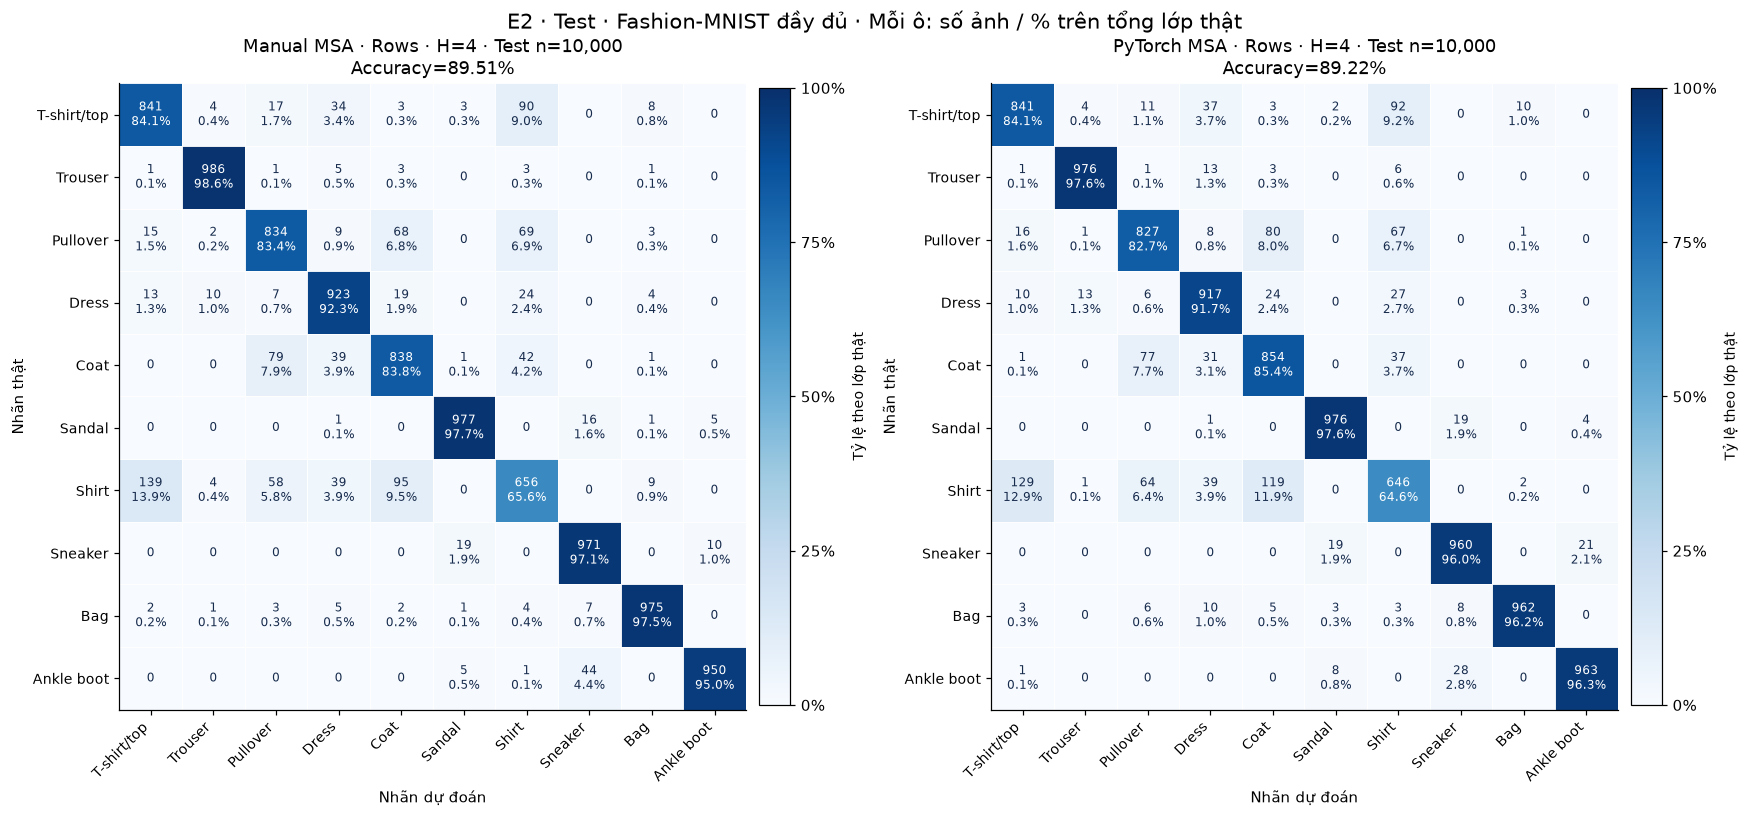
\includegraphics[width=.98\linewidth,height=.67\textheight,keepaspectratio]{assets/e2/confusion_test_pair_1.png}
\caption{E2: confusion matrix test, cặp1; tên model ghi trên từng panel.}\end{figure}\end{landscape}
\begin{landscape}\begin{figure}[p]\centering
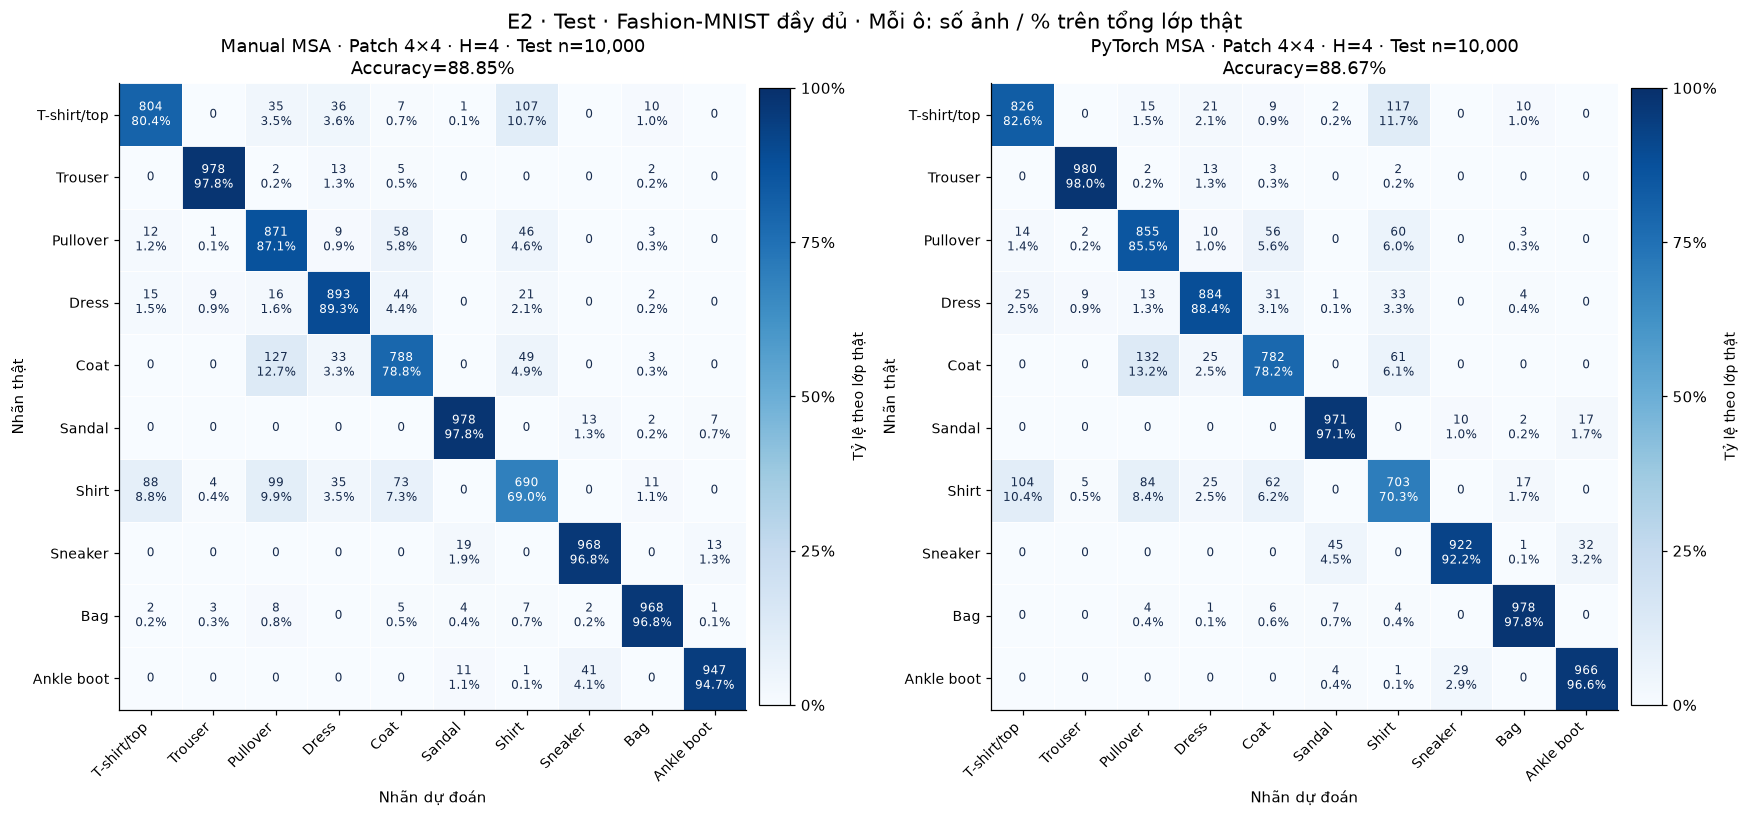
\includegraphics[width=.98\linewidth,height=.86\textheight,keepaspectratio]{assets/e2/confusion_test_pair_2.png}
\caption{E2: confusion matrix test, cặp2; tên model ghi trên từng panel.}\end{figure}\end{landscape}
\begin{landscape}\begin{figure}[p]\centering
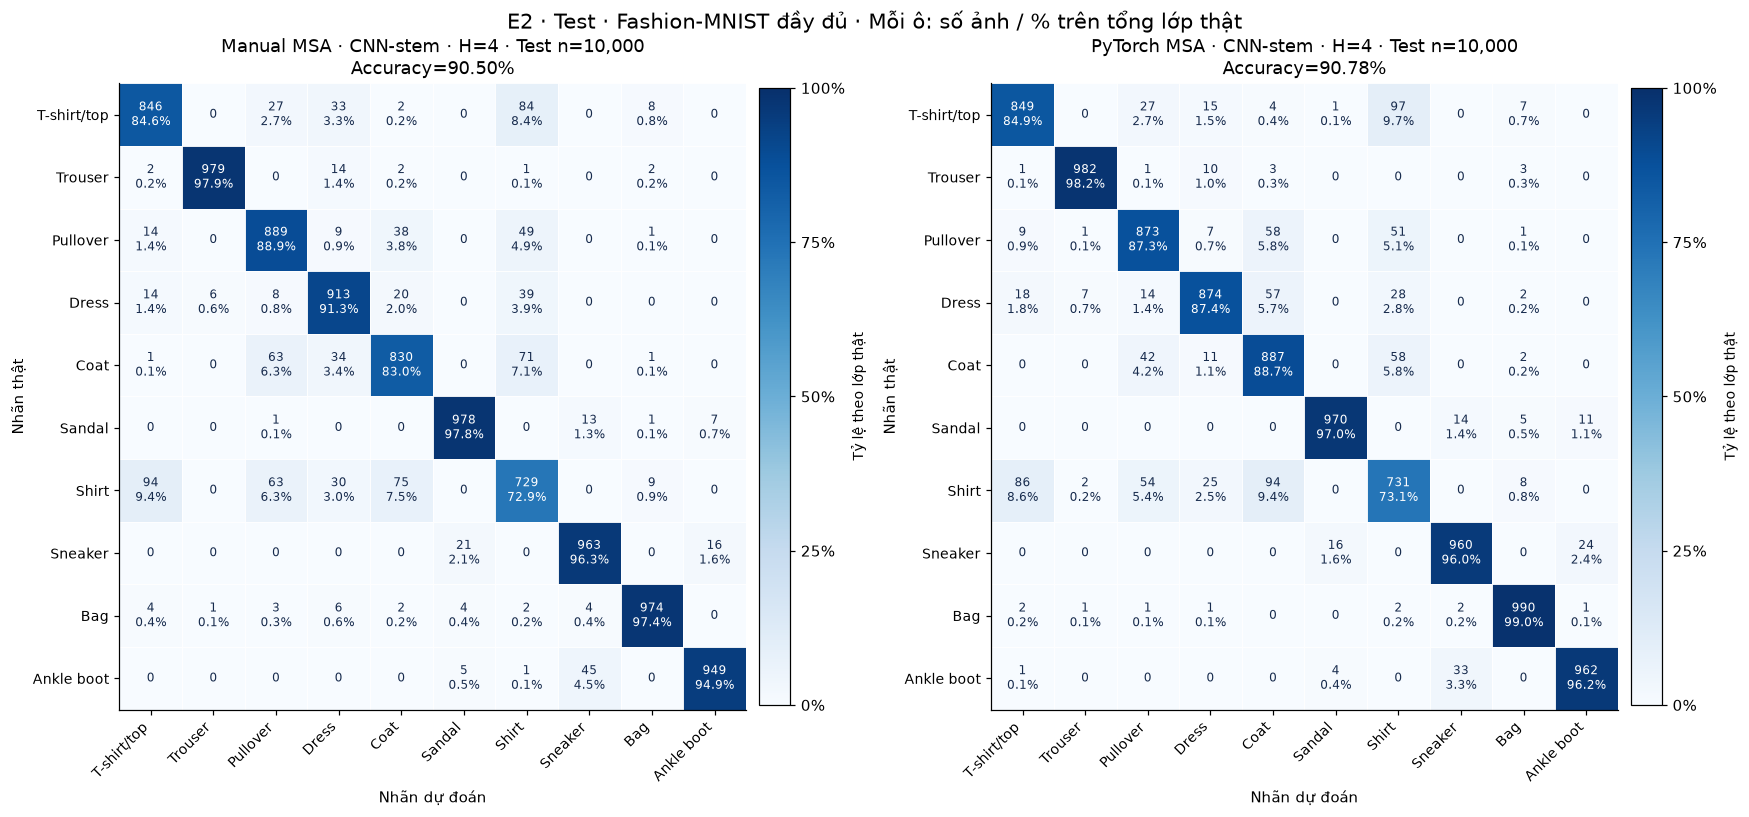
\includegraphics[width=.98\linewidth,height=.86\textheight,keepaspectratio]{assets/e2/confusion_test_pair_3.png}
\caption{E2: confusion matrix test, cặp3; tên model ghi trên từng panel.}\end{figure}\end{landscape}
\begin{landscape}\begin{figure}[p]\centering
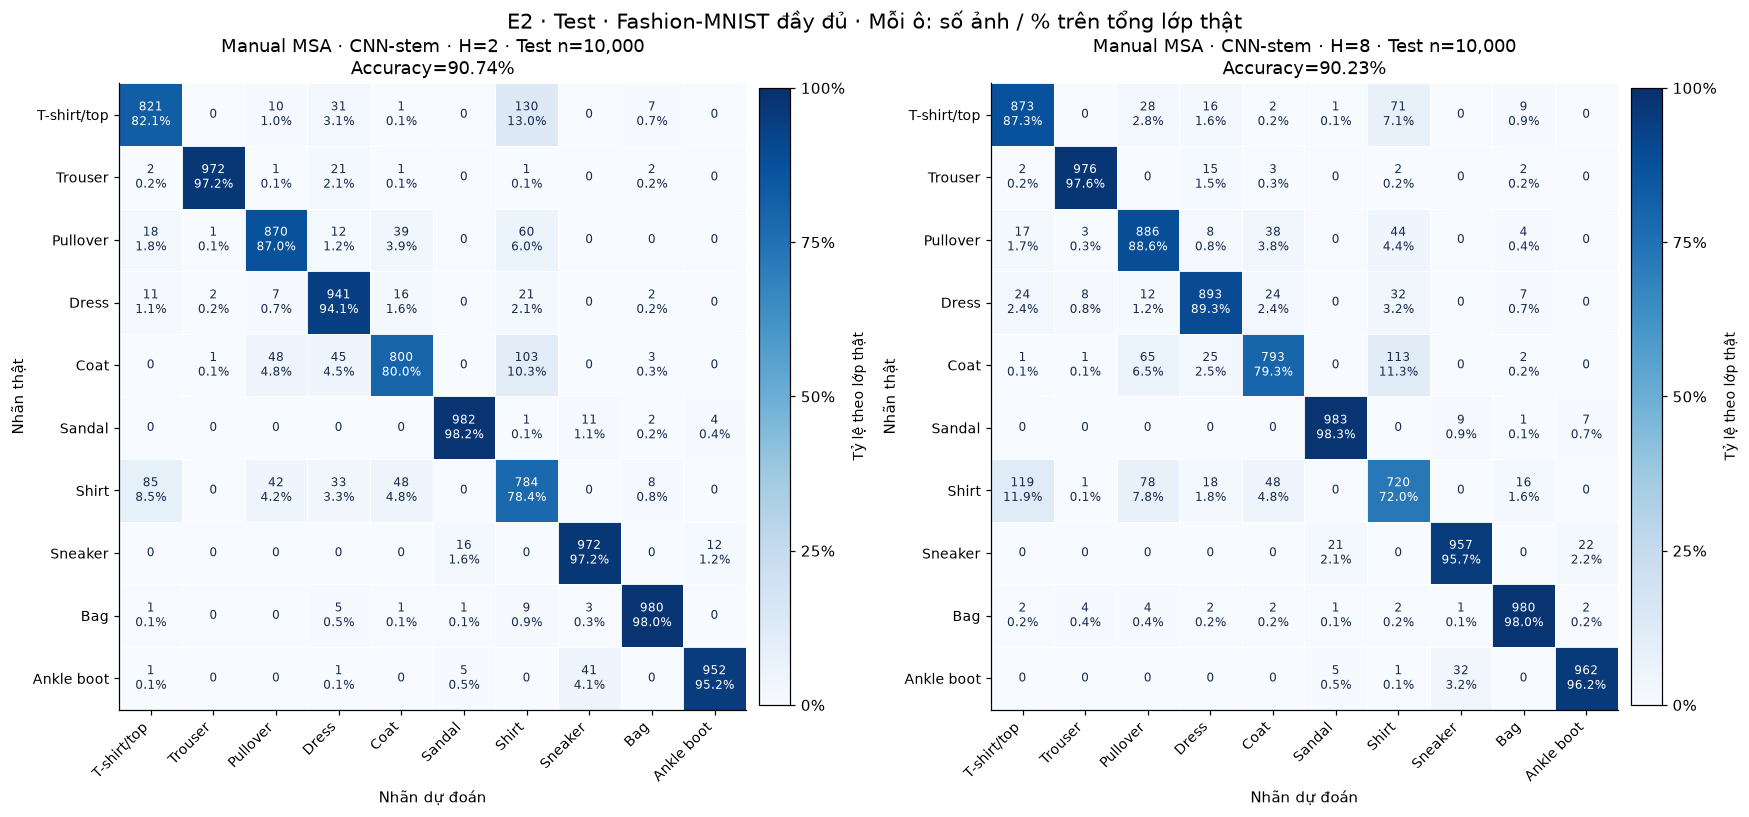
\includegraphics[width=.98\linewidth,height=.86\textheight,keepaspectratio]{assets/e2/confusion_test_pair_4.png}
\caption{E2: confusion matrix test, cặp4; tên model ghi trên từng panel.}\end{figure}\end{landscape}
\begin{landscape}\begin{figure}[p]\centering
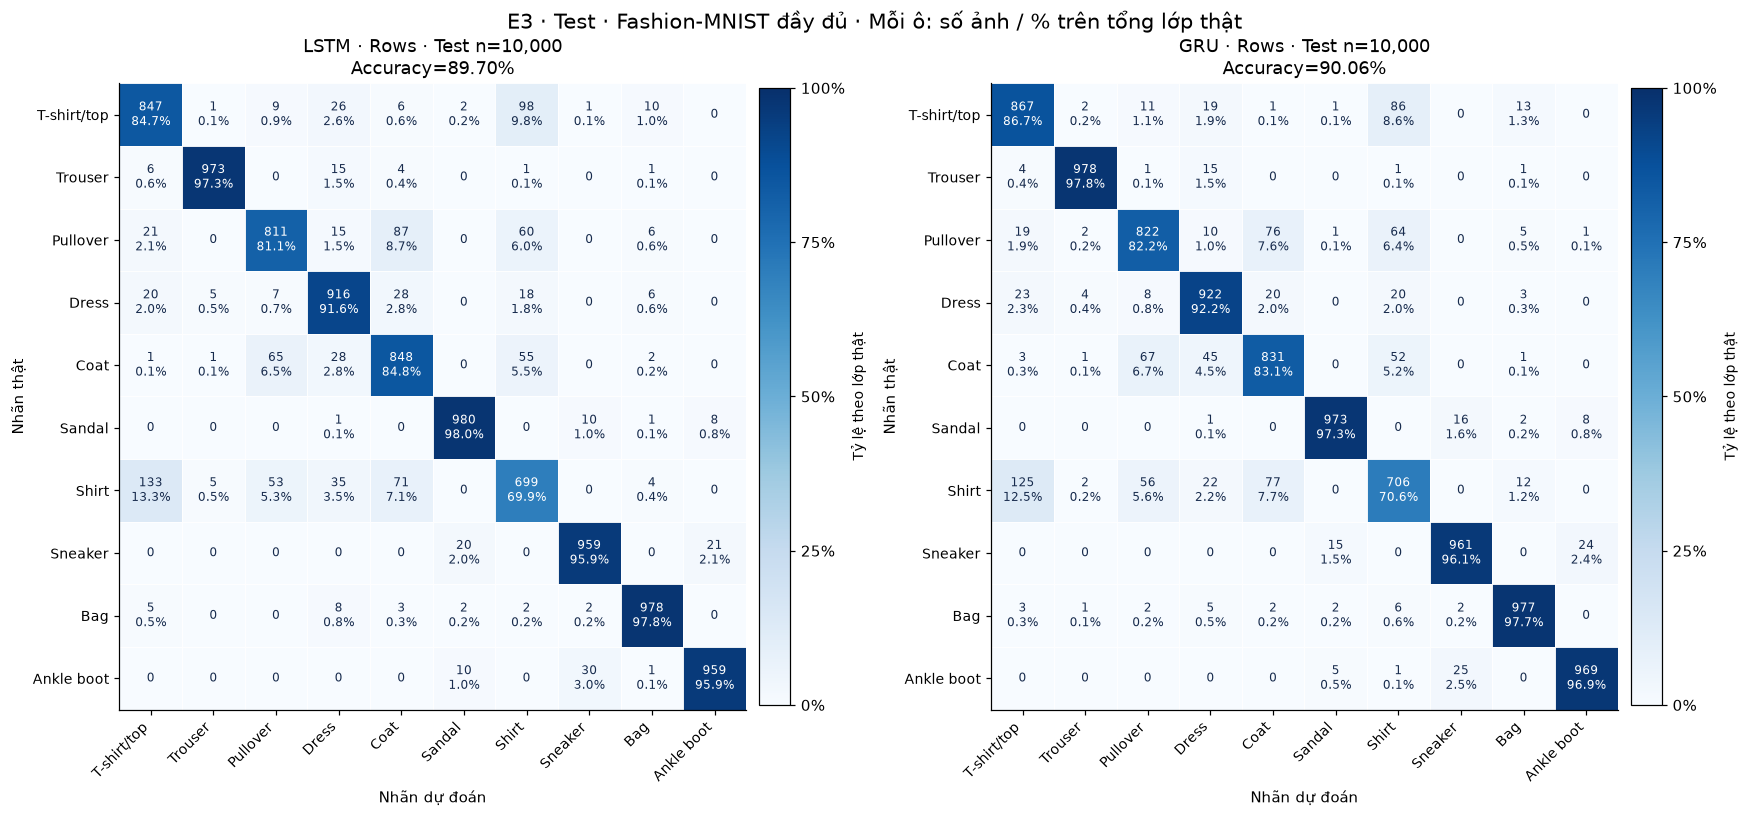
\includegraphics[width=.98\linewidth,height=.86\textheight,keepaspectratio]{assets/e3/confusion_test_pair_1.png}
\caption{E3: confusion matrix test, cặp1; tên model ghi trên từng panel.}\end{figure}\end{landscape}
\begin{landscape}\begin{figure}[p]\centering
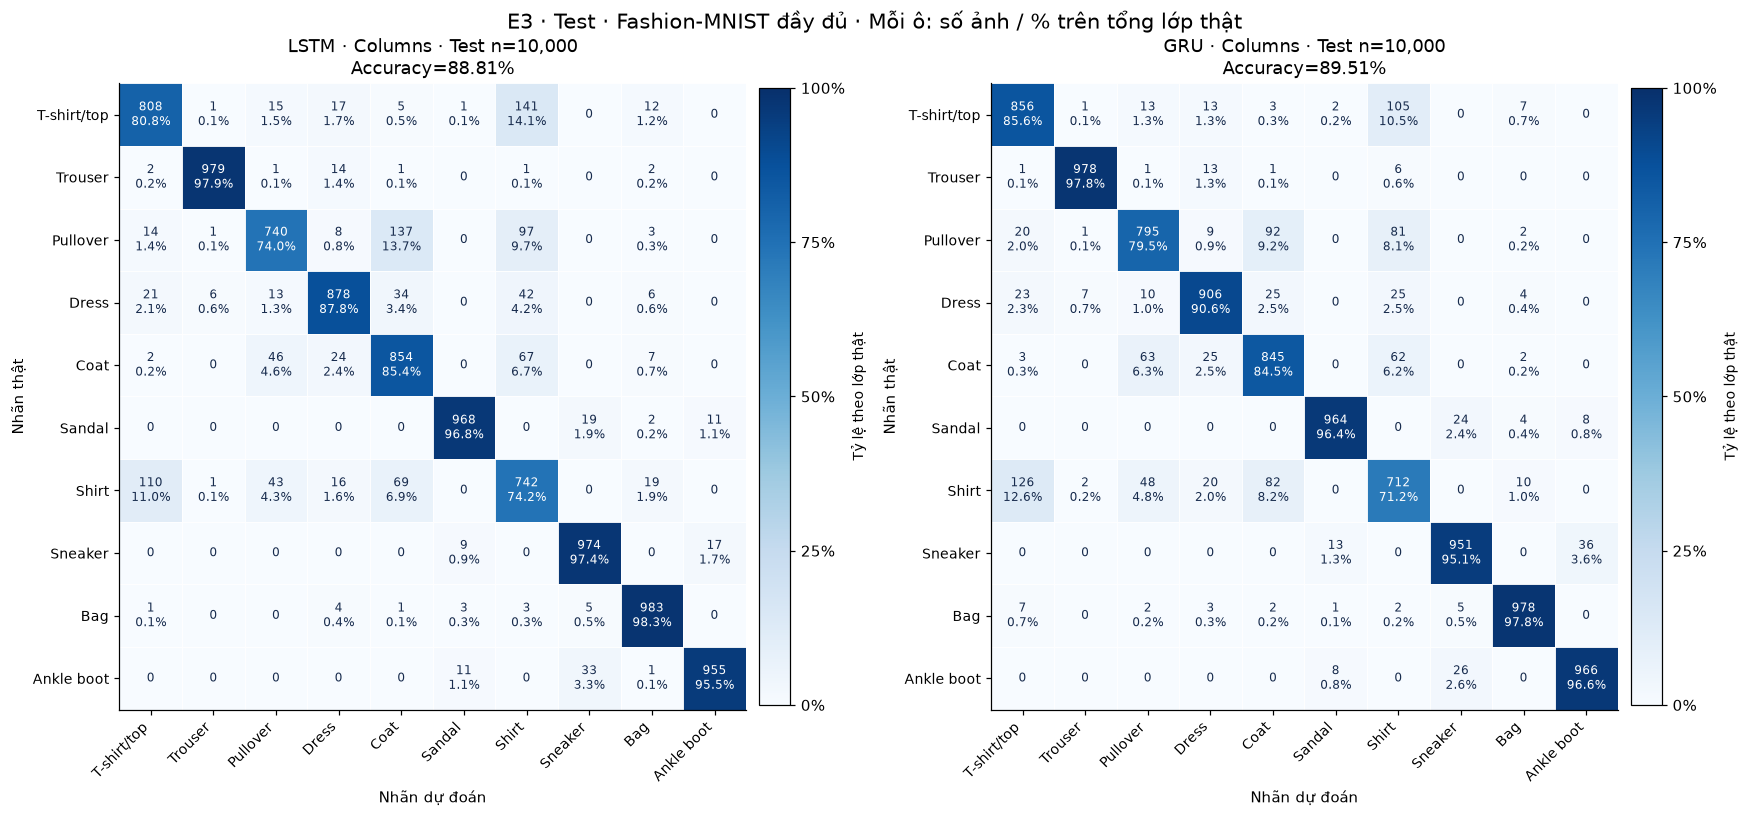
\includegraphics[width=.98\linewidth,height=.86\textheight,keepaspectratio]{assets/e3/confusion_test_pair_2.png}
\caption{E3: confusion matrix test, cặp2; tên model ghi trên từng panel.}\end{figure}\end{landscape}
\begin{landscape}\begin{figure}[p]\centering
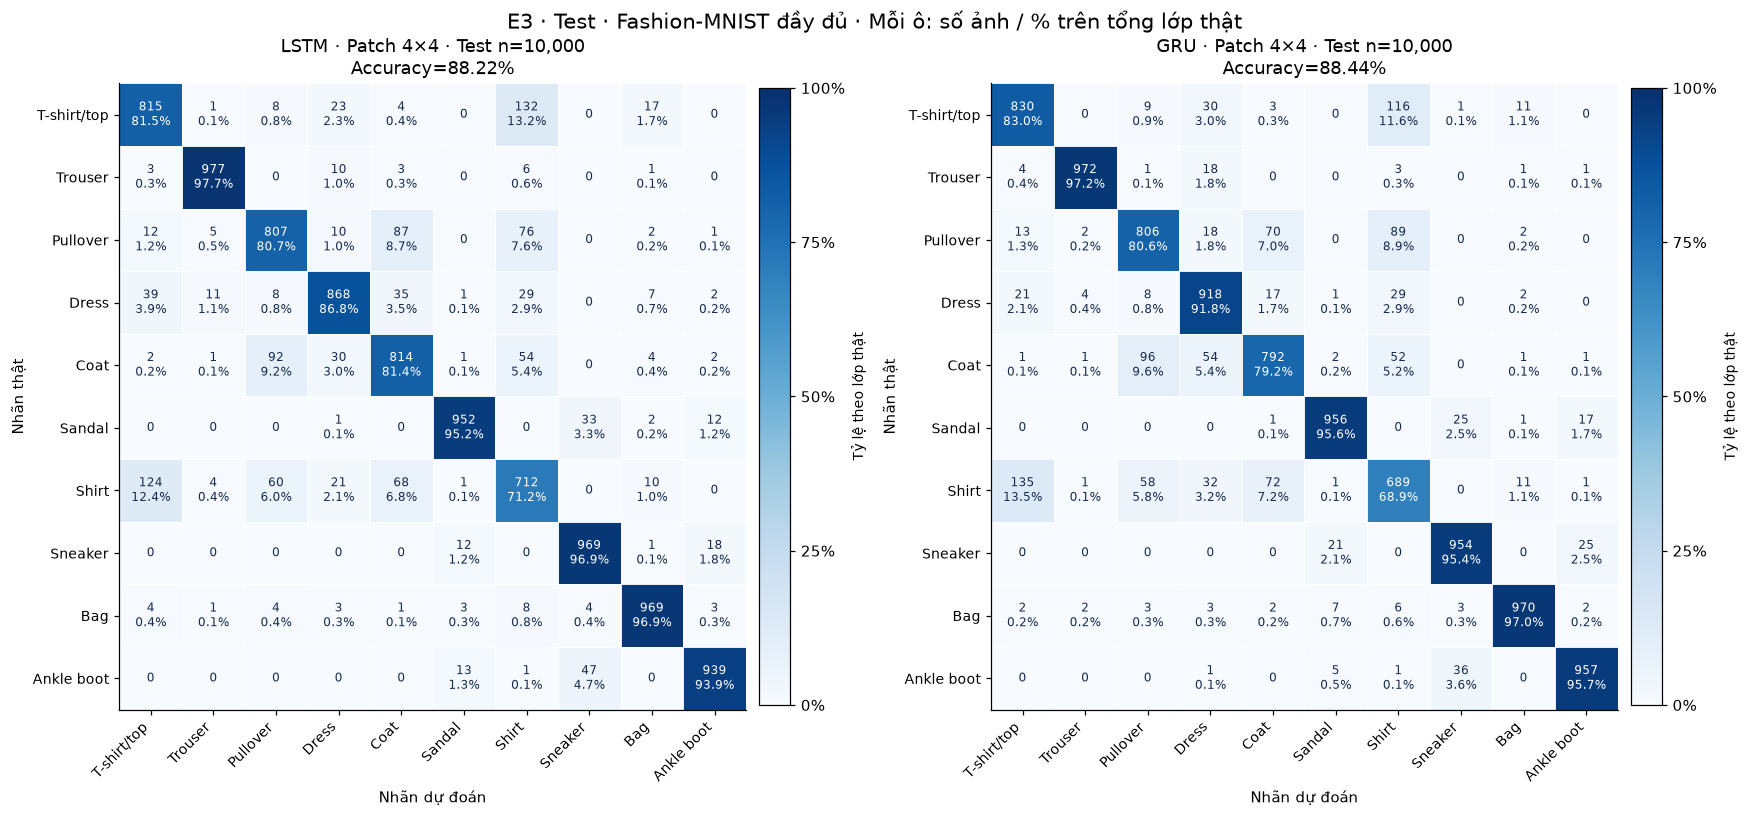
\includegraphics[width=.98\linewidth,height=.86\textheight,keepaspectratio]{assets/e3/confusion_test_pair_3.png}
\caption{E3: confusion matrix test, cặp3; tên model ghi trên từng panel.}\end{figure}\end{landscape}
\begin{landscape}\begin{figure}[p]\centering
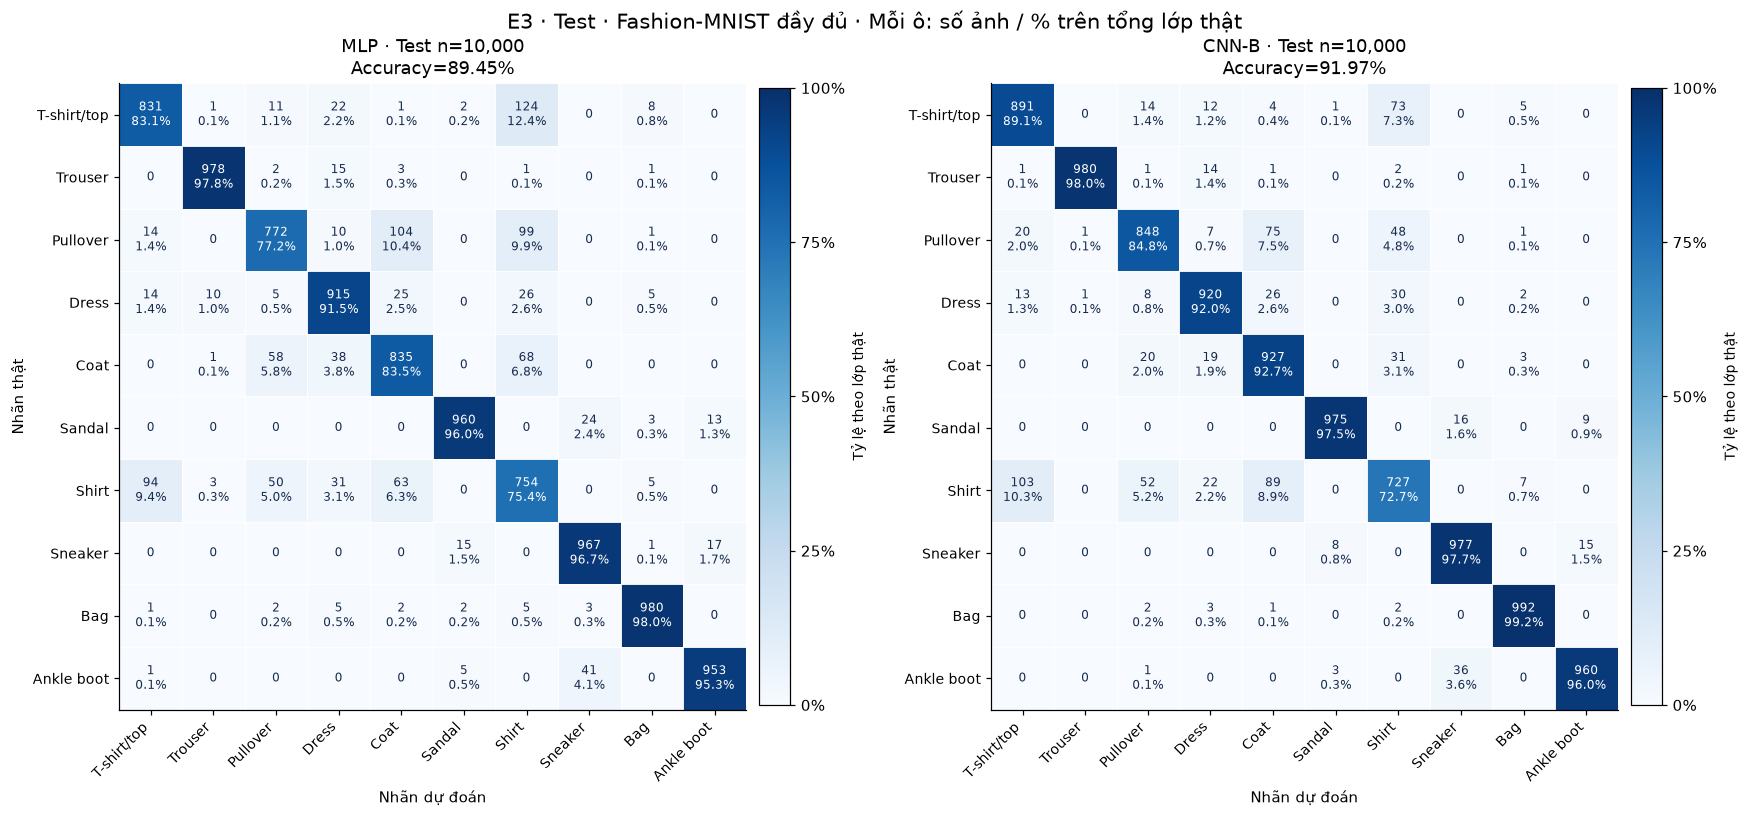
\includegraphics[width=.98\linewidth,height=.86\textheight,keepaspectratio]{assets/e3/confusion_test_pair_4.png}
\caption{E3: confusion matrix test, cặp4; tên model ghi trên từng panel.}\end{figure}\end{landscape}

\section{Nguồn số liệu và hướng dẫn tái lập}
Nguồn số liệu là output đã lưu của E1.ipynb, E2.ipynb, E3.ipynb và A1.ipynb
trong source\_code. Manifest dưới assets/e1, e2, e3, a1 ghi cell/output và
bảng Markdown nguồn; PNG trích từ ảnh embedded trong notebook, không chạy
training để tạo lại số liệu. Notebook không tự ghi assets của báo cáo.

Chuẩn bị dữ liệu theo README trong thư mục datasets. Mở notebook tương ứng,
chọn Python 3.14 có CUDA, Restart Kernel và Run All, sau đó Save. Mỗi notebook
chạy độc lập; không cần thứ tự. Để tái hiện đúng số liệu lịch sử E1--E3,
cần dùng cấu hình patience10 ghi trong output; mặc định code hiện tại là 4.
A1 sử dụng patience 4 như số liệu đã báo cáo. Seed cố định không đảm bảo
tái lập bitwise qua mọi GPU, phiên bản thư viện hoặc đường thực thi AMP.

Báo cáo biên dịch bằng XeLaTeX và BibTeX từ report/source\_latex/main.tex;
các sơ đồ kiến trúc là mã TikZ trong từng chương, ảnh kết quả nằm ở assets.
Sản phẩm PDF chung giữ tại report/CO5085\_Report.pdf.

\end{document}
